\section{Results}
\label{sec:results}

\subsection{Verifier choice reverses orderings}
\label{sec:results-census}

The two verifiers disagree on \nNDisagree{} of \nNRows{} responses
(\nDisRate{}, 95\% CI [\nDisLo, \nDisHi]; \nEmOnly{} credited only by
\code{exact\_match}, \nSbOnly{} only by \code{score\_boxed}), from \nDisMin{}
to \nDisMax{} per model. Table~\ref{tab:reversals} lists the \nScorerFlips{}
orderings that reverse between them. \nScorerFlipsCmdr{} involve
\code{c4ai-command-r-v01}, which \code{exact\_match} scores at 0. The audit
contains few items per model, but in each case its evidence points the same
way: \code{command-r-v01}'s responses credited only by \code{score\_boxed}
are mostly wrong, as are \code{Yi-1.5-9B-Chat}'s (most commit to no answer),
while \code{zephyr-orpo} and \code{Qwen2-7B}'s are correct.

\begin{table}[t]
  \centering
  \caption{Orderings that reverse between the two verifiers. ``Sampling-clear'':
  the accuracy difference exceeds 1.96 standard errors under the named
  verifier(s). Last column: audited responses credited only by
  \code{score\_boxed} whose transcribed answer is correct, for each model.}
  \label{tab:reversals}
  \scriptsize
  \resizebox{\linewidth}{!}{\begin{tabular}{@{}lllcc@{}}
\toprule
Pair & higher by score\_boxed & higher by exact\_match & sampling-clear & audited sb-only correct/n \\
\midrule
Yi-1.5-9B-Chat vs zephyr-orpo-141b-A35b-v0.1 & Yi-1.5-9B-Chat & zephyr-orpo-141b-A35b-v0.1 & both & 1/9 ; 2/2 \\
Yi-1.5-9B-Chat vs Qwen2-7B & Yi-1.5-9B-Chat & Qwen2-7B & em only & 1/9 ; 2/2 \\
c4ai-command-r-v01 vs gpt-j-6b & c4ai-command-r-v01 & gpt-j-6b & both & 2/6 ; 0/0 \\
c4ai-command-r-v01 vs phi-2 & c4ai-command-r-v01 & phi-2 & both & 2/6 ; 0/0 \\
c4ai-command-r-v01 vs Mistral-7B-v0.1 & c4ai-command-r-v01 & Mistral-7B-v0.1 & both & 2/6 ; 0/0 \\
c4ai-command-r-v01 vs mpt-7b & c4ai-command-r-v01 & mpt-7b & both & 2/6 ; 0/0 \\
c4ai-command-r-v01 vs falcon-40b & c4ai-command-r-v01 & falcon-40b & both & 2/6 ; 0/0 \\
c4ai-command-r-v01 vs falcon-7b & c4ai-command-r-v01 & falcon-7b & both & 2/6 ; 0/1 \\
\bottomrule
\end{tabular}
}
\end{table}

\subsection{Per-model correction with one verifier resolves nothing}
\label{sec:results-single}

With \code{score\_boxed} and each model's own audited items, the audit finds
\nFalseCredits{} false credits in \nNCredAud{} credited items and \nFalseMiss{}
false rejections in \nNWrongAud{} rejected ones, and corrected point
estimates reorder only \nPointFlips{} pairs. Yet at 95\% coverage the audit
resolves \nSingleComb{} orderings, against \nCeiling{} that sampling error
alone permits (Appendix~\ref{sec:appendix-single}, Figure~\ref{fig:intervals}).
\nRShare{} of each model's interval width comes from the rejected stratum:
zero observed errors in 1--17 items bounds $r_m$ only loosely, and the
rejected stratum holds most of each model's responses. Simulated
single-verifier audits resolve half the orderings at about \nLabelsEight{}
labels (Appendix~\ref{sec:appendix-single}). Plug-in Neyman allocation
resolves none at any budget, because zero-event pilot strata receive no
labels.

\subsection{Where verifier error concentrates}
\label{sec:results-cells}

\begin{table}[t]
  \centering
  \caption{Audited responses of the \nNModels{} models by joint verifier cell,
  and how many have a transcribed answer equal to the reference (responses
  committing to no answer count as not equal).}
  \label{tab:cells}
  \small
  \begin{tabular}{@{}lcccc@{}}
    \toprule
    Cell & both credit & both reject & \code{score\_boxed} only & \code{exact\_match} only \\
    \midrule
    Audited & \nCellElevenN & \nCellZeroN & \nCellTenN & \nCellZeroOneN \\
    Transcription correct & \nCellElevenX & \nCellZeroX & \nCellTenX & \nCellZeroOneX \\
    \bottomrule
  \end{tabular}
\end{table}

Where the verifiers agree, the transcribed answer disagrees with them on
\nConcErr{} of \nConcN{} audited responses; the exact 95\% upper bound on
this rate is \nConcUpper{} (\nElevenUpper{} and \nZeroUpper{} for the two
concordant cells separately). This is a low observed rate with a finite-sample
bound, not proof that agreement is reliable, and it says nothing about
whether the rate is the same for every model. Where \code{score\_boxed}
credits and \code{exact\_match} does not, \nCellTenX{} of \nCellTenN{}
transcriptions are correct (Table~\ref{tab:cells}); every false credit of
\code{command-r-v01} is in this cell. The \code{exact\_match}-only cell has
493 responses in the population but \nCellZeroOneN{} audited, because the
audit was stratified on \code{score\_boxed}.

\subsection{What verifier agreement buys, and what it assumes}
\label{sec:results-joint}

\begin{figure}[t]
  \centering
  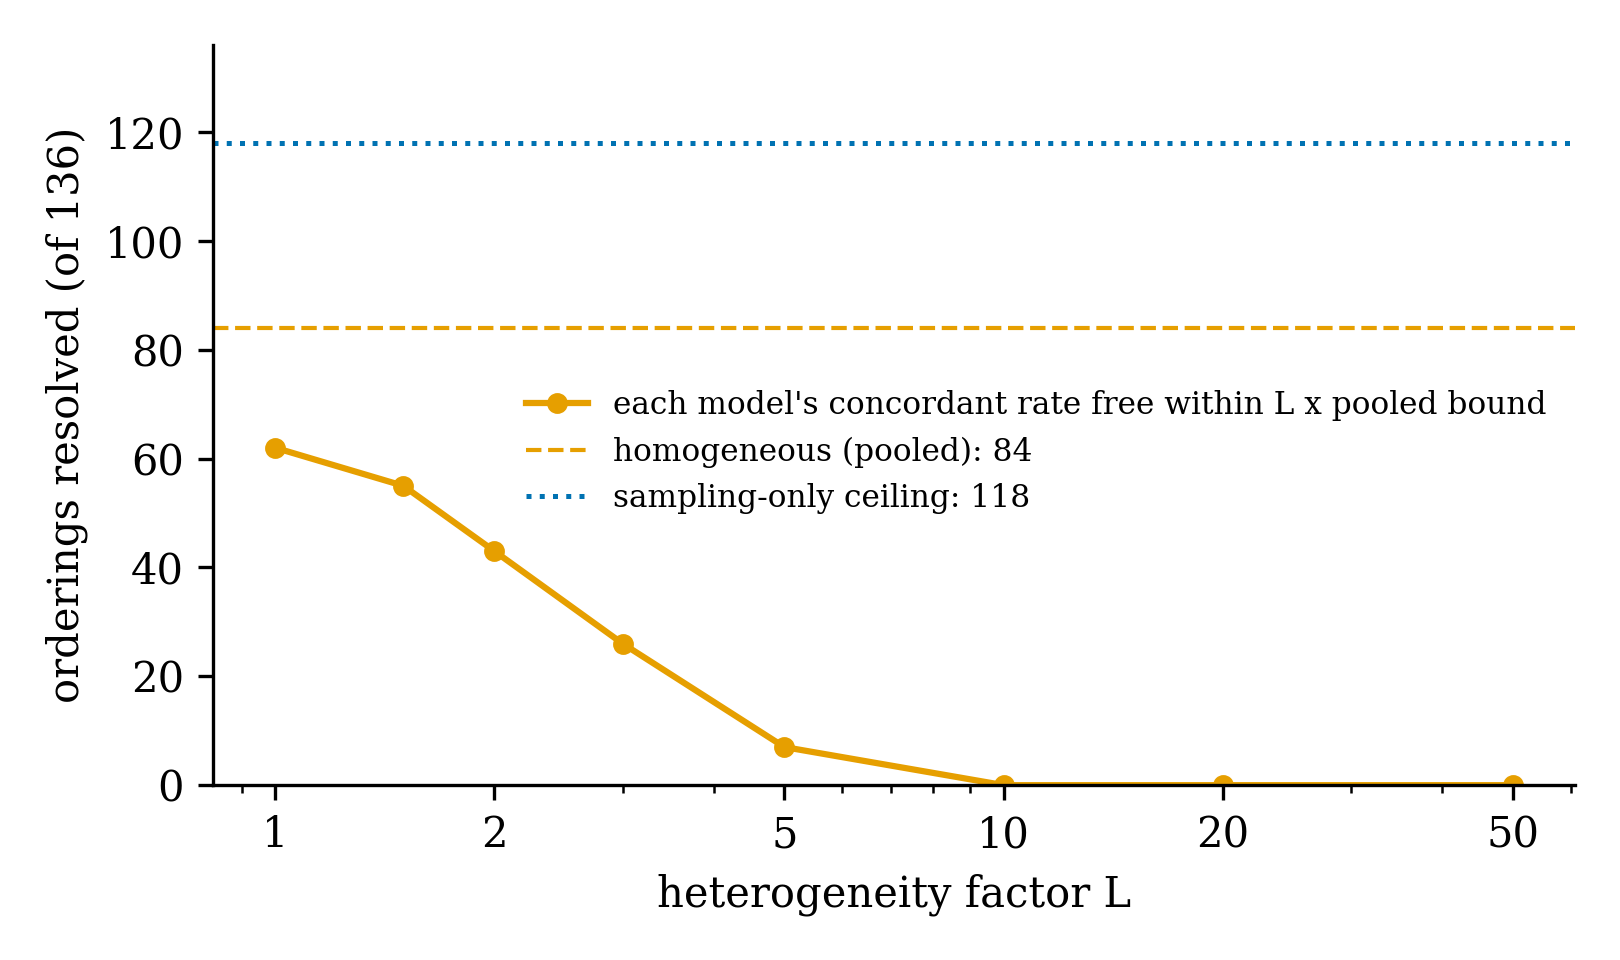
\includegraphics[width=0.66\linewidth]{figE_homogeneity_sensitivity.png}
  \caption{Orderings resolved by the existing audit, at 95\% coverage per
  ordering, as the concordant-cell assumption is relaxed. Dashed: concordant
  error homogeneous across models. Solid: each model's concordant error free
  within $L$ times the pooled bound. Dotted: orderings that sampling error
  alone permits.}
  \label{fig:assumption}
\end{figure}

Under homogeneity, with disagreement cells left model-specific and bounded
only by $[0,1]$, the existing audit resolves \nJointComb{} of the \nCeiling{}
orderings sampling permits (\nJointAudit{} of \nNPairs{} from the audit
alone; \nJointSim{} of \nCeilingSim{} with coverage simultaneous over all
orderings; \nJointCombDrop{} if responses without a committed answer are
dropped rather than counted as incorrect). Figure~\ref{fig:assumption} shows
how much of this is the assumption. If each model's concordant error may lie
anywhere within the pooled bound ($L=1$), \nHetOne{} orderings remain; at
$L=2$, \nHetTwo; at $L=5$, \nHetFive; at $L=10$, \nHetTen. With no pooling at
all the count is \nNoPool{}. Recovering \nJointComb{} without the assumption
would require about \nNPLabelsFull{} concordant labels (\nNPThreeK{} at
3{,}400), because every model's two concordant cells, which hold most of its
responses, would need their own tight bounds.

The assumption is plausible on mechanism: two extractors that read answers
in different ways and return the same verdict rarely both err on the same
response. The audit cannot confirm it model by model: models have 0 to 37
audited items per concordant cell.

\subsection{Designing the next audit}
\label{sec:results-design}

\begin{figure}[t]
  \centering
  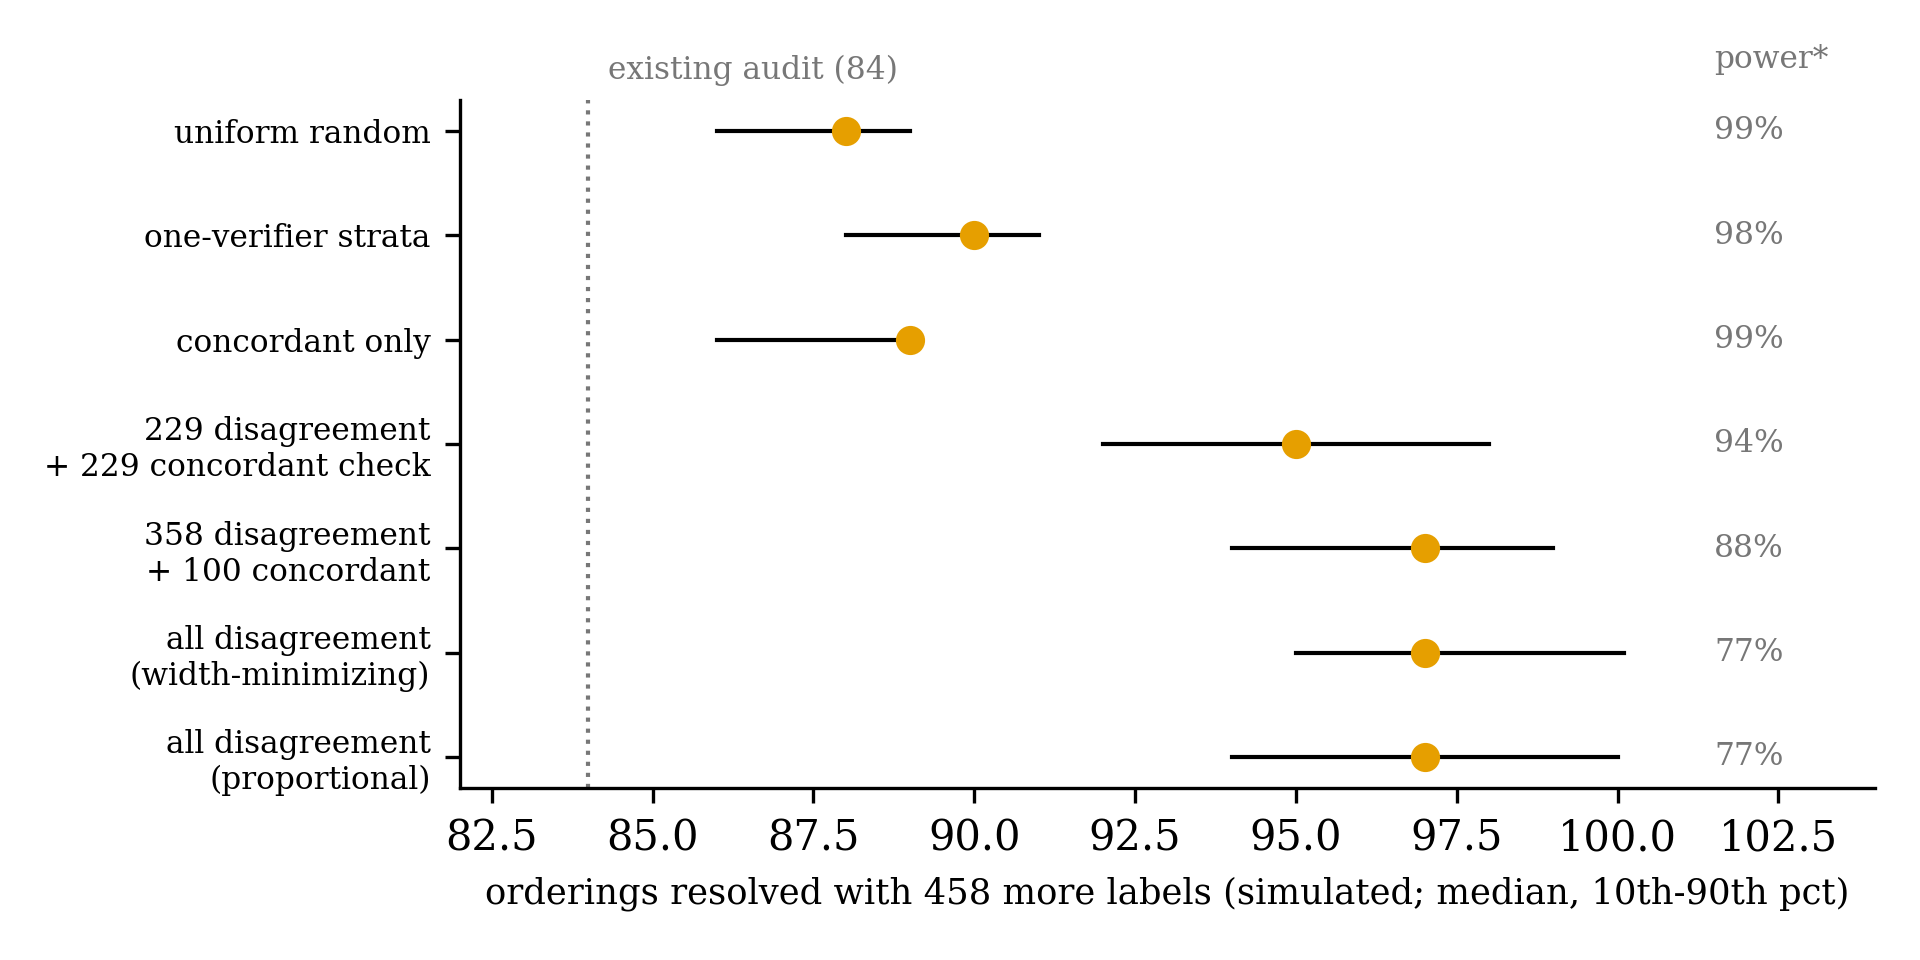
\includegraphics[width=0.80\linewidth]{figD_design_comparison.png}
  \caption{Projected, not observed. Orderings resolved (homogeneous analysis)
  after 458 further labels under each design; \nNRep{} simulated audits per
  design, truths drawn from the existing audit's posterior; median and
  10th--90th percentile. Right column (*): median across models of the
  probability of observing at least one concordant error for a model whose
  concordant error rate is 10\%.}
  \label{fig:designs}
\end{figure}

Figure~\ref{fig:designs} compares designs for 458 further labels under the
same objective. Under homogeneity, spending most labels on disagreements
gives a median of \nDesFullMin--\nDesFullMax{} resolved orderings across
truth scenarios, against \nDesUniform{} for uniform sampling and \nDesOneVer{}
for one-verifier strata; allocations within the disagreement cells differ by
at most a few orderings, so none is uniquely best. The same designs differ
sharply in how well they test the assumption the result rests on: an
all-disagreement design would detect a model with a 10\% concordant error
rate with median probability \nPowFull{} (worst model \nPowFullMin), a
half-and-half design with \nPowBalanced{} (\nPowBalancedMin) while still
reaching \nDesBalancedMin--\nDesBalancedMax. We preregistered the
half-and-half design: 229 disagreement responses stratified by model and 229
concordant responses spread evenly over models. These results are projections
from simulations that draw truths from the same audit used to choose the
design; they are not observed outcomes.
